\newpage % Rozdziały zaczynamy od nowej strony.

\section{Opis zastosowanego rozwiązania}
W przypadku wykorzystywania sieci splotowych wraz z sieciami rekurencyjnymi, w celu stworzenia architektury zajmującej się generowaniem podpisów do obrazów, najczęstszym typem połączenia tychże dwóch modułów jest wykorzystanie wartości wyjściowej sieci splotowej jako pierwszego elementu sekwencji przetwarzanej przez sieć rekurencyjną. Jest to niezwykle proste rozwiązanie, przy pomocy którego możliwe jest osiągnięcie sensownych rezultatów. Głównym problemem takiego podejścia jest uwzględnienie jedynie informacji końcowej generowanej przez sieć splotową. Pomijany jest ogrom danych przetwarzanych w warstwach pośrednich. Sieć rekurencyjna mogłaby znacząco skorzystać na uwzględnieniu wartości przetwarzanych w pośrednich warstwach splotowych, których wynikiem są tak zwane mapy szczegółów. Zawierają one kontekst informacji znajdujących się na obrazie o różnym poziomie uszczegółowienia.

W celu zaadresowania tego problemu oraz wykorzystania informacji, jakie generuje sieć splotowa w wyższych warstwach, w niniejszej pracy zostało wykorzystane zmodyfikowane rozwiązanie łączące moduły kodujący i dekodujący z uwzględnieniem danych z pośrednich warstw splotowych modułów kodujących.

Macierze generowane przez pośrednie warstwy splotowe zostały wyciągnięte, spłaszczone, zredukowane i połączone w jeden wektor, co pozwoliło na wykorzystanie go jako wartości wejściowej dla sieci rekurencyjnej. Takie rozwiązanie umożliwia uwzględnienie wartościowych danych, które mogą mieć istotne znaczenie dla ostatecznego wyniku.

Wektory pochodzące z warstw splotowych, otrzymane poprzez ich spłaszczenie są zbyt długie, by mogły być wykorzystane jako wartości wejściowe dla sieci rekurencyjnej, dlatego konieczna jest ich redukcja. W tym celu wykorzystane zostały warstwy w pełni połączone, które również są wykorzystywane w ostatnich warstwach sieci splotowej. Taki zabieg pozwala na otrzymanie ostatecznego wektora o pożądanej długości z zachowaniem istotnych informacji pochodzących z map szczegółów. Dużym minusem takiego podejścia jest konieczność dodatkowych obliczeń przeprowadzanych przez warstwy w pełni połączone. W celu ograniczenia zwiększania zużycia zasobów obliczeniowych, dla każdej mapy szczegółów została wykorzystana tylko jedna warstwa w pełni połączona. Takie podejście może nie być optymalny -- wektory map szczegółów są znaczącej długości, a przy redukcji poprzez tylko jedną warstwę w pełni połączoną może dojść do utraty dużej części informacji, jednakże znacząco ograniczy to zużycie zasobów obliczeniowych. Dodatkowo takie rozwiązanie pozwoli sprawdzić, w jakim stopniu pojedyncze warstwy w pełni połączone wpływają na wydajność generowania podpisów, jak również skuteczność. Schemat modułu kodującego został przedstawiony na rysunku \ref{fig:schemat-probkowanie}.
\begin{figure}[H]
    \centering
    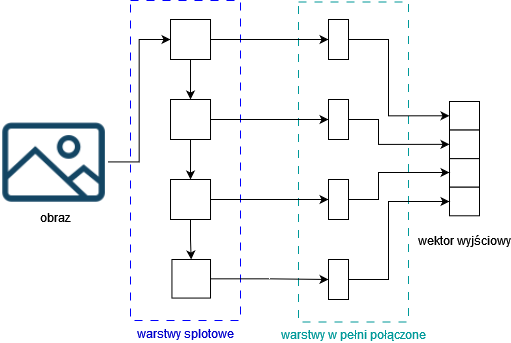
\includegraphics[width=\linewidth]{diagram_probkowanie}
    \caption{Diagram przedstawiający architekturę modułu kodującego. Opracowanie własne}
    \label{fig:schemat-probkowanie}
\end{figure}
\noindent Każdy wektor wyjściowy warstwy splotowej został zredukowany do takiego samego rozmiaru, który wyniósł 1024. Następnie zostały one połączone w jeden wektor, który posłużył jako wartość wejściowa modułu dekodującego. Schemat przedstawia jedynie poglądowy sposób działaniu modułu kodującego. Ze względu na wykorzystanie wielu różnych sieci splotowych w ramach modułu kodującego, mapy szczegółów zostały wydobyte na różnych ich poziomach.
\subsection{AlexNet}
Sieć AlexNet \cite{alexnet} składa się z kilku warstw zawierających następujące elementy:
\begin{itemize}
    \item warstwa splotowa,
    \item funkcja aktywacji ReLU,
    \item warstwa redukująca.
\end{itemize}
Warstwa redukująca następnie jest połączona ponownie z warstwą splotową. Cała sieć zawiera pięć takich bloków. Wartości wyjściowe z warstw redukujących zostały wykorzystane jako wektory wejściowe dla warstw w pełni połączonych, których wyjście tworzy ostateczny wektor wyjściowy. Jako że ostateczny wektor składa się jedynie z czterech wektorów składowych, przedostatni blok został pominięty.
% MAYBE: diagram alexnet
\subsection{VGG}
Sieć VGG \cite{vggnet} posiada nieco bardziej rozbudowaną architekturę niż sieć AlexNet. Podstawowe bloki również składają się z warstwy splotowej, funkcji aktywacji ReLU oraz warstwy redukcyjnej, jednakże główną różnicą jest zastosowanie większej ilości warstw splotowych w późniejszych poziomach całej sieci, co można zaobserwować na rysunku \ref{fig:vgg-diagram}.
\begin{figure}[H]
    \centering
    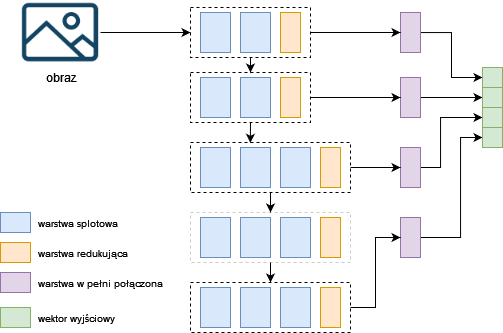
\includegraphics[width=\linewidth]{vgg_diagram}
    \caption{Diagram przedstawiający architekturę sieci VGG. Opracowanie własne.}
    \label{fig:vgg-diagram}
\end{figure}
\noindent Pierwsze dwa bloki są złożone z dwóch warstw splotowych, natomiast kolejne z trzech. Z takiej konfiguracji można wyodrębnić pięć głównych bloków, tak samo, jak w przypadku sieci AlexNet. W celu utworzenia ostatecznego wektora wyjściowego pominięty został przedostatni blok.
% MAYBE: diagram vgg
\subsection{ResNet}
Architektura ResNet \cite{resnet} znacząco odbiega swoją budową od poprzednich sieci. Posiada ona cztery główne bloki składające się z pomniejszych bloków, które z kolei zawierają trzy warstwy splotowe wraz z warstwami normalizującymi. W celu utworzenia wektora wyjściowego nie było konieczności pomijania żadnego bloku ze względu na to, iż architektura składa się z czterech zasadniczych bloków. Pozwoliło to na utworzenie ostatecznego wektora składającego się z danych pochodzących z czterech różnych warstw sieci ResNet.
% MAYBE: diagram resnet
\subsection{GoogleNet}
Sieć GoogleNet \cite{googlenet} podobnie do pozostałych sieci splotowych składa się z kilku bloków posiadających różne konfiguracje warstw splotowych. Elementem rozpoznawalnym tejże sieci jest blok Inception. Sieć posiada aż 9 takich bloków. Wektor wyjściowy został utworzony z map szczegółów pochodzących z bloków pierwszego, trzeciego, szóstego oraz dziewiątego. Taki wybór w najlepszy sposób uwzględnia różne poziomy szczegółowości obrazu -- od najbardziej ogólnych pochodzących z wczesnych etapów sieci do najbardziej szczegółowych.
% MAYBE: diagram resnet
\subsection{Klasyczne podejście}
W celu sprawdzenia skuteczności zastosowanego rozwiązania zostało ono porównane z klasycznym połączeniem modułu kodującego z dekodującym. W tym przypadku dane wyjściowe pochodzące z sieci splotowej zostały wykorzystane jako pierwszy element sekwencji wejściowej sieci rekurencyjnej. W celu osiągnięcia takowego połączenia konieczna była modyfikacji architektury sieci splotowych przedstawiona na rysunku \ref{fig:schemat-pretrained}.
\begin{figure}[H]
    \centering
    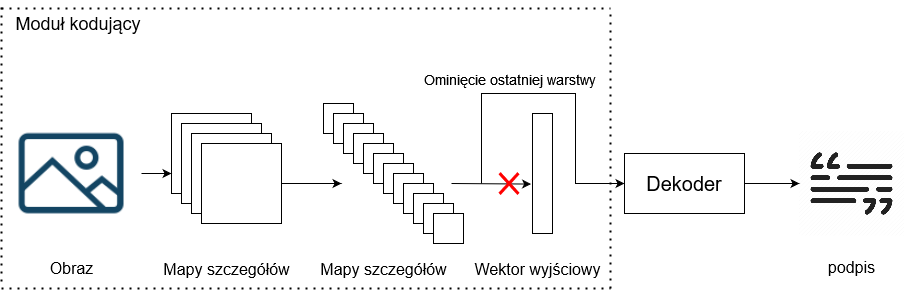
\includegraphics[width=\linewidth]{schemat-pretrained}
    \caption{Diagram przedstawiający architekturę wykorzystującą klasyczne połączenie modułów kodującego oraz dekodującego. Opracowanie własne.}
    \label{fig:schemat-pretrained}
\end{figure}
\noindent Z architektury sieci splotowej została usunięta ostatnia warstwa odpowiedzialna za przekształcenie danych do ostatecznego wektora odpowiadającego klasom rozpoznawanych obiektów. Takie podejście ograniczające modyfikację modułu kodującego jedynie do ostatniej warstwy pozwala wykorzystać ich wstępnie wytrenowane wagi poprzez tak zwaną technikę transferu wiedzy.
\subsection{Transfer wiedzy}
Szeroką popularnością w dziedzinie trenowania modeli sieci neuronowych cieszy się technika przenoszenia wiedzy. Jest to technika uczenia maszynowego, w której model uczony jest na jednym zadaniu, a następnie wykorzystuje tę wiedzę do lepszego rozwiązania innego, zazwyczaj podobnego zadania. Może zostać ona podzielona na dwa kluczowe kroki:
\begin{itemize}
    \item Początkowe uczenie modelu na dużym zbiorze danych i zadaniu, na którym jest dostępna duża ilość informacji.
    \item  Dostosowanie modelu do nowego zadania. Parametry modelu są dostosowywane do specyfiki nowego zadania, a wagi nauczone podczas początkowe uczenia są używane jako punkt wyjścia.
\end{itemize}
W przypadku generowania podpisów do obrazków technikę przenoszenia wiedzy można zastosować poprzez wykorzystanie wcześniej wyuczonych modeli sieci splotowych w ramach modułu kodującego. Trenowanie splotowych sieci neuronowych od zera na dużym zbiorze danych może być czasochłonne i wymagać dużej ilości zasobów obliczeniowych. Wykorzystanie wstępnie wytrenowanych modeli pozwala uniknąć tego procesu, ponieważ modele te są już przeszkolone do ekstrakcji cech, co jest ich głównym zadaniem w całej architekturze. Z tego względu dane treningowe zostały poddane wcześniejszemu przetworzeniu przez moduł kodujący, a trening polegał na uczeniu jedynie modułu dekodującego w przypadku rozwiązania wykorzystującego proste połączenie między modułami. Rozwiązanie angażujące dodatkowe warstwy w pełni połączone wymaga również ich wyuczenia, jednakże architektura została skomponowana w ten sposób, aby nie ingerowała w wewnętrzną strukturę sieci splotowych, a co za tym idzie, transfer wiedzy również w tym przypadku może zostać wykorzystany.
